\chapter{Ergebnisse}   \label{ch_4}
Im folgenden Kapitel werden die durchgeführten statistischen Berechnungen dargestellt. Zu Beginn werden die deskriptiven Ergebnisse beschrieben und mit den Normwerten verglichen, woraufhin die statistische Überprüfung der Manipulation folgt. Im inferenzstatistischen Unterkapitel wird mit der Prüfung der Vorraussetzung der einzelnen Test mathematisch dargestellt und abschließend werden die Ergebnisse der drei Hypothesen präsentiert. Die ausführliche Interpretation der Ergebnisse geschieht im nachkommenden Kapitel ~\ref{ch_5}. 
Wie zuvor erklärt, musste der Datensatz verdoppelt werden, um eine Berechnung mit den Daten gewährleisten zu können. Aus diesem Grund wird in diesem und den nachfolgenden Kapiteln von einer Stichprobengröße von $N_{neu}$~=~864 ausgegangen.

\section{Deskriptive Ergebnisse}    \label{sec_4.1}
Die Fallvignetten wießen, bei einem $Min$~=~1 und einem $Max$~=~101, einen Mittelwert von $M$~=~26.46 ($SD$~=~27.98) auf. Der Median lag bei $Mdn$~=~19. Die am häufigsten verteilten Werte liegen an den beiden Extremen bei 1.00 und 101.00 und bilden eine bimodale Verteilung. Bei einer Schiefe von 1.17 und Kurtosis von 0.53, liegt eine rechstschiefe beziehungsweise. linkssteile und steilgipflige Verteilung vor. Abbildung~\ref{Histogramm VicBlame} stellt die unimodale Verteilung der Verantwortungszuschreibung bildlich da. Die vorhandenen Ausreißer befinden sich alle unter der Ausscheidungsgrenze.
% Modus: 1.00 und 101.00
\begin{figure}[htb]
    \centering
        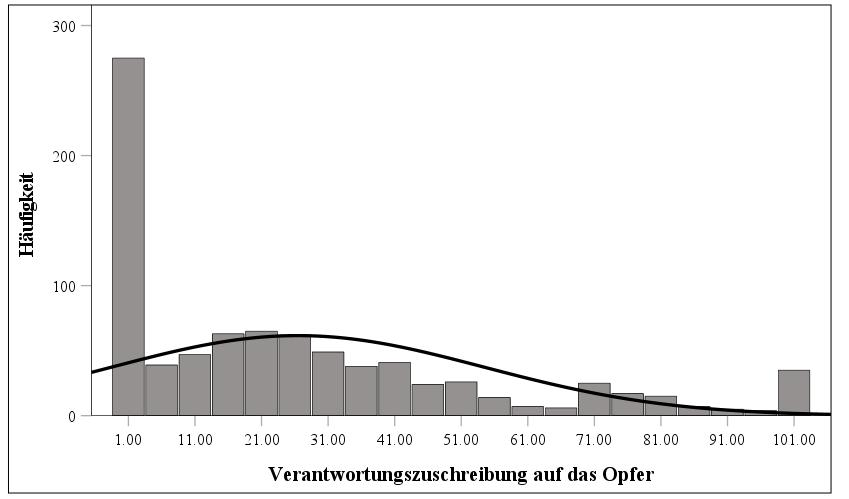
\includegraphics[width=0.8\linewidth]{Histogramm VicBlame.jpg}
        \caption[Histogramm Verantwortungszuschreibung]{Verteilung der Verantwortungszuschreibung.}
        \label{Histogramm VicBlame}
\end{figure}



Der DVMAS zeigte einen Mittelwert von $M$~=~2.60 ($SD$~=~0.80) und einen Median von $Mdn$~=~2.5. Der geringste Wert war dabei $Min$~=~1 und der höchsete $Max$~=~5.56. Die häufigsten Werte lagen bei 2.11 und 2.67 und bilden eine bimodale Verteilung. Eine Schiefe von 0.60 bildet eine leicht rechstschiefe Verteilung. Die Kurtosis von 0.09 bildet eine leicht steilere Verteilung, als die Normalverteilung. Beide Werte weichen demzufolge leicht von einer Normalverteilung ab ($M$~=~2.30, $SD$~=~0.85 und Schiefe~=~0.63). 
Die Abbildung~\ref{Histogramm DVMAS} bildet die beschriebenen Werte dieser Studie bildlich ab. Die vorhandenen Ausreißer befinden sich alle unter der Ausscheidungsgrenze.
% Modus: 2.11, 2.67
\begin{figure}[htb]
    \centering
        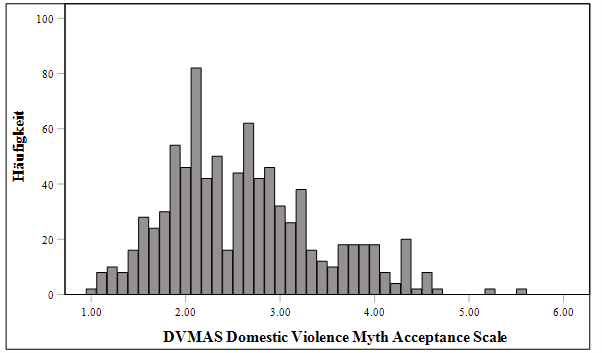
\includegraphics[width=0.8\linewidth]{Histogramm - DVMAS.png}
        \caption[Histogramm Altersverteilung]{Verteilung der Akzeptanz von Gewaltmythen.}
        \label{Histogramm DVMAS}
\end{figure}



\begin{figure}[htb!]
    \centering
        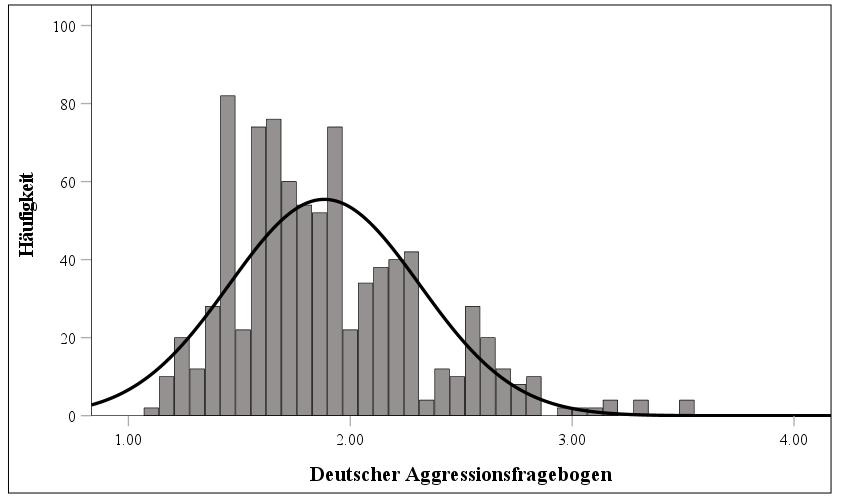
\includegraphics[width=0.8\linewidth]{Histogramm AggroFB.jpg}
        \caption[Histogramm Aggressionsfragebogen]{Verteilung der Angaben des Aggressionsfragebogens.}
        \label{Histogramm AggroFB}
\end{figure}


Beim Deutschen Aggressionsfragebogen wurde ein Mittelwert von $M$~=~1.88 ($SD$~=~0.43) und ein Median von $Mdn$~=~1.79 berechnet. Der geringste angegebene Wert betrug $Min$~=~1.10 und der höchste $Max$~=~3.52. Die Verteilung wies einen Schiefe von 0.94 und eine Kurtosis von 0.88 auf. Demzufolge ist die Verteilung rechstschiefe und hat eine breitgipflige Form, sowie eine Multimodalität mit den Modiwerten bei 1.59, 1.62, 2.52 und 2.55. Die Lageparameter weichen stark von den Normwerten ab. Diese sind wie folgt: $M$~=~2.66 ($SD$~=~0.88), Schiefe~=~3.81 und eine Kurtosis von -0.06. In Abbildung~\ref{Histogramm AggroFB} ist eine bildliche Darstellung der erhobenen Verteilung zu sehen. Die vorhandenen Ausreißer befinden sich alle unter der Ausscheidungsgrenze.
% Modus: 1.59, 1.62, 2.52, 2.55


\section{Inferenzstatistische Ergebnisse}    \label{sec_4.2}
Anschließend erfolgt eine inferenzstatistische Analyse der erhobenen Daten zur Fesstellung der Korrelationen zwischen den in Kapitel~\ref{ch_2} näher gebrachten Konstrukte Aggression, Akzeptanz der Gewaltmythen und die Verantwortungszuschreibung. 


\subsection{Hypothese 1}    \label{subsec_4.2.1}
Die Hypothese 1 geht von einer Korrelation des Aggressionsscores mit Victim Blaming aus. Diese ungerichtete Zusammenhangshypothese wurde mit der Spearman$-$Rang$-$Korrelation berechnet. Die in Kapitel ~\ref{sec_3.5} erwähnten Voraussetzungen der Ordinalität beider Variablen wie auch die paarweise Beobachtungen sind gegeben. Eine gepaarte Beobachtung entspricht einer gemessenen Variable pro Spalte bei SPSS.
\begin{table}[htb]
    \caption[Mittelwerte, Standardabweichung und Korrelation von Aggression und Victim Blaming]{\textit {Mittelwerte, Standardabweichung und Korrelation von Aggression und Victim Blaming}} 
    \label{H1_Spearman}
    \centering
    \begin{adjustbox}{width=6.5cm} %{maxwidth=\textwidth}
    \small
    \begin{tabular}{lrrr}
      \hline
        & $M$   & $SD$ & 1 \\
      \hline
    1 Aggression      & 1.88  & 0.43   & $-$      \\
    2 Victim Blaming  & 26.46 & 27.98  & .18      \\
       \hline
    \end{tabular}
    \end{adjustbox}
    
    \begin{tablenotes}
        \item \textit{Anmerkungen.} \( N_{neu} \)~=~864; Wertebereich der Variable Aggression 1 (\textit{trifft nicht zu}) bis 4 (\textit{trifft voll zu}); Spearman$-$Rang$-$Korrelation.
      \end{tablenotes}
    \end{table}



Das in Tabelle~\ref{H1_Spearman} ersichtliche Ergebnis der Spearman$-$Rang$-$Korrelation fiel nicht signifikant aus ($p$~=~n.s.). Mit dem sehr kleinen Effekt \parencite{Cohen_1992} von $r_{s}$~=~.18, korreliert die Aggression nur sehr gering mit der Verantwortungszuschreibung auf das Opfer.

\subsection{Hypothese 2}    \label{subsec_4.2.2}
Die Voraussetzung einer Pearson$-$Produkt$-$Moment$-$Korrelation wurden in ~\ref{sec_3.5} bereits aufgeführt. In diesem Falle sind auch alle Voraussetzungen gegeben: Aggression und die Akzeptanz von Gewaltmythen sind metrisch, die vorhandenen Ausreißer sind im akzeptablen Bereich (siehe Anhang~\ref{Boxplot_AggroFB} und Anhang~\ref{Boxplot_DVMAS}), 
es liegt ein linearer Zusamenhang zwischen den Variablen vor (siehe Anhang~\ref{Linearitat_AggroFB_DVMAS}) und eine bivariate Normalverteilung ist auch gegeben, da der Bootstrap$-$Konfidenzintervall (.308 $-$ .442) die Null nicht einbezieht.

Die in Tabelle~\ref{H2_Pearson} ersichtliche Pearson$-$Produkt$-$Moment$-$Korrelation zeigte einen Zusammenhang von $r$~=~.38. Nach \textcite{Cohen_1992} entspricht dies einer mittelgroßen Korrelation, die bei einseitiger Testung statistisch signifikant ausfiel ($p<$ .001).
\begin{table}[htb]
    \caption[Mittelwerte, Standardabweichung und Korrelation von Aggression und der Akzeptanz von Gewaltmythen]{\textit {Mittelwerte, Standardabweichung und Korrelation von Aggression und der Akzeptanz von Gewaltmythen}} 
    \label{H2_Pearson}
    \centering
    \begin{adjustbox}{width=5.5cm} %{maxwidth=\textwidth}
    \small
    \begin{tabular}{lrrr}
      \hline
        & $M$   & $SD$ & 1 \\
      \hline
    1 Aggression      & 1.88 & 0.43  & $-$      \\
    2 DVMAS           & 2.60 & 0.80  & .38*      \\
       \hline
    \end{tabular}
    \end{adjustbox}
    
    \begin{tablenotes}
        \item \textit{Anmerkungen.} \( N_{neu} \)~=~864; DVMAS = Akzeptanz der Gewaltmythen; Wertebereich der Variable Aggression 1 (\textit{trifft nicht zu}) bis 4 (\textit{trifft voll zu}); Variable DVMAS 1 (stimme überhaupt nich zu) bis 7 (stimme völlig zu); Pearson$-$Produkt$-$Moment$-$Korrelation. \\ *$p<$~.001
      \end{tablenotes}
    \end{table}




\subsection{Hypothese 3}    \label{subsec_4.2.3}
Um die vermutete Moderation des biologischen Geschelchts auf den Zusammenhang zwischen Aggressio und dem DVMAS zu testen, wurde eine Moderationsanalyse durchgeführt. Die Variablen weisen eine lineare Beziehung und eine Unabhängigkeit, durch die nicht verbundene Erhebung der einzelnen Variablen, auf. Durch die mit $N_{neu}$~=~864 großen Stichprobe, kann von einer Normalverteilung der Residuen ausgegangen werden. Die Überprüfung der Homoskedastizität mithilfe des White$-$Tests ergab eine signifikantes Ergebnis ($p$~=~.03). Somit liegt eine Heteroskedastizität vor. 

\begin{table}[htb]
    \caption[Moderationsanalyse Geschlecht und Aggression auf die Akzeptanz von Gewaltmythen]{\textit {Moderationsanalyse Geschlecht und Aggression auf die Akzeptanz von Gewaltmythen}} 
    \label{Moderationsanalyse}
    \centering
    \begin{adjustbox}{width=11cm} %{width=\textwidth}
    \small
    \begin{tabular}{lrrrrr}
      \hline
      & $B$    & $SE(B)$  & $t$    & $p$ & $\Delta R^{2}$\\
      \hline
    Konstante  & 2.59    & 0.03 & 103.13  & $<$~.001 & \\
    Aggression & 0.68    & 0.06 & 11.13   & $<$~.001 & \\
    Geschlecht & $-$0.24 & 0.05 & $-$4.32 & $<$~.001 & \\
    Interaktionsterm & $-$0.14 & 0.13 & $-$1.06 & .290 & .001 \\
    $R^{2}$          &         &      &         &      & .163* \\
       \hline
    \end{tabular}
    \end{adjustbox}
    
    \begin{tablenotes}
        \item \textit{Anmerkungen.} \( N_{neu} \)~=~864; *$p<$~.001
      \end{tablenotes}
    \end{table}




Das Gesamtmodell war, wie in Tabelle~\ref{Moderationsanalyse} demonstriert, mit einer Varianzaufklärung von 16.34\% signifikant ($F$(3, 856)~=~50.30, $p<$ .001). Die Moderationsanalyse konnte jedoch keinen signifikanten Moderationseffekt finden, $\Delta R^{2}$~=~0.12\%, F(1, 860)~=~1.12, $p$~=~.290, 95\% CI[-0.39, 0.12]. Dennoch klärt das Modell 16.34\% der Varianz des deutschen DVMAS auf.
%Modell: $R^{2}$~=~16.34\%, $F$(HC3)~=~50.30, $df1$~=~1, $df2$~=~856 $p<$~.001
%W*X: $\Delta R^{2}$~=~0.08, $F$(HC3)~=~0.76, $df1$~=~1, $df2$~=~856 $p$~=~.384

\begin{table}[htb]
    \caption[Modell mit Haupteffekten]{\textit {Modell mit Haupteffekten}} 
    \label{Haupteffekte}
    \centering
    \begin{adjustbox}{width=10.5cm} %{width=\textwidth}
    \small
    \begin{tabular}{lrrrrr}
      \hline
               & $B$    & $SE(B)$ & \textbeta  & $t$    & $p$ \\
      \hline
    Geschecht  & $-$.23 & 0.06    & $-$.13   & 4.191  & $<$~.001 \\
    Aggression & .69    & 0.06    & .37      & 11.842 & $<$~.001 \\
       \hline
    \end{tabular}
    \end{adjustbox}
    
    \begin{tablenotes}
        \item \textit{Anmerkungen.} \( N \) = 864%; *$p<$~.001
      \end{tablenotes}
    \end{table}


Den Entfehlungen von \textcite{Moderation_SPSS} folgend, wurde der Interaktionsterm herausgenommen. Dies führte zu einem neuen Modell mit Haupteffekten, welche in Tabelle~\ref{Haupteffekte} zusammengefasst wurden. Die Beziehung zwischen Geschlecht ($B$~=~$-$.23, $p<$~.001), wie auch zwische Aggression ($B$~=~.69, $p<$~.001) und der Akzeptanz von Gewaltmythen fiel signifikant aus. 
%Geschlecht: $B$~=~$-$.23, $(SE)B$~=~0.06, $\beta$~=~$-$.13, $t$~=~$-$4.191, $p<$~.001
%Aggression: $B$~=~.69, $(SE)B$~=~0.06, $\beta$~=~.37, $t$~=~11.842, $p<$~.001


\section{Manipulationscheck}    \label{sec_4.3}
Nachfolgend werden die Ergebnisse der vier Manipulationschecks in der folgenden Reihenfolge aufgeführt: Gewaltart, Geschlecht des Opfers, soziökonomischer Status der betroffenen Person und abschließend der Kulturelle Hintergrund.


\begin{table}[htb]
    \caption[Kreuztabelle Manipulationscheck Gewaltart]{\textit {Kreuztabelle des Manipulationschecks der Gewaltart}} 
    \label{KT_G}
    \centering
    \begin{adjustbox}{width=10cm} %{width=\textwidth}
    \small
    \begin{tabular}{lrrr}
      \hline
        &   & psychische Gewalt & sexualisierte Gewalt \\
      \hline
    Ja   & Anzahl  & 32      & 354     \\
         & Prozent & 8.30\%  & 91.70\% \\
    Nein & Anzahl  & 400     & 78      \\
         & Prozent & 83.70\% & 16.30\% \\
       \hline
    \end{tabular}
    \end{adjustbox}
    
    \begin{tablenotes}
        \item \textit{Anmerkungen.} \( N \) = 864. Prüffrage: Ging es um sexualisierte Gewalt?
      \end{tablenotes}
    \end{table}
\begin{table}[htb]
    \caption[Kreuztabelle Manipulationscheck Opfergeschlecht]{\textit {Kreuztabelle des Manipulationschecks des Geschlecht der betroffenen Person}} 
    \label{KT_sex}
    \centering
    \begin{adjustbox}{width=\textwidth}
    \small
    \begin{tabular}{lrrr}
      \hline
        &   & weibliches Opfer & männliches Opfer \\
      \hline
    Ja   & Anzahl  & 411      & 14      \\
         & Prozent & 96.70\%  & 3.30\%  \\
    Nein & Anzahl  & 16       & 423     \\
         & Prozent & 3.60\%   & 96.40\% \\
       \hline
    \end{tabular}
    \end{adjustbox}
    
    \begin{tablenotes}
        \item \textit{Anmerkungen.} \( N \) = 864. Prüffrage: War das Opfer eine Frau?
      \end{tablenotes}
    \end{table}
Bei der Überprüfung der Gewaltart gaben bei Vignetten sexualisierter Gewalt 354 Personen (91.70\%) an eine solche Gewaltart behandelt zu haben. Handelte es sich um eine psychische Gewaltart an, reichten nur 400 Personen (83.70\%) die richtige Antwort ein. Der durchgeführte Chi$^2$-Test viel mit einem Wert von 485.53 signifikant aus ($p<$.001). 
In Tabelle~\ref{KT_G} sind die Werte dieser Manipulationsprüfung nochmals zusammengefasst.

War die Nachfrage auf das Geschlecht des Opfers gerichtet gaben die 411 (96.70\%) bzw. 423 (96.40\%) Probanden an, es handelte sich um ein weibliches bzw. männliches Opfer. Auch dieser Chi$^2$-Test war mit einem Wert von 748.16 hoch signifikant ($p<$.001). 
In Tabelle~\ref{KT_sex} sind die Werte dieser Manipulationsprüfung nochmals zusammengefasst.

Die Überprüfung des niedrigen soziökonomischen Status des Opfers wurde von 389 (80.2\%) bei dessen Gegebenheit richtig beanwortet. Bei der gegenteiligen Situation stieg die Rate der richtigen Antworten auf 342 (90.20\%). Mit einem Wert von 422.37 fiel dieser Chi$^2$-Test ebenfalls signifikant aus ($p<$.001). 
In Tabelle~\ref{KT_SES} sind die Werte dieser Manipulationsprüfung nochmals zusammengefasst.
\begin{table}[htb]
    \caption[Kreuztabelle Manipulationscheck soziökonomischer Status des Opfers]{\textit {Kreuztabelle des Manipulationschecks des soziökonomischen Status der betroffenen Person}} 
    \label{KT_SES}
    \centering
    \begin{adjustbox}{width=10cm} %{width=\textwidth}
    \small
    \begin{tabular}{lrrr}
      \hline
        &   & niedriger SES Opfer & hoher SES Opfer \\
      \hline
    Ja   & Anzahl  & 389      & 96      \\
         & Prozent & 80.20\%  & 19.8\%  \\
    Nein & Anzahl  & 37       & 342     \\
         & Prozent & 9.80\%   & 90.20\% \\
       \hline
    \end{tabular}
    \end{adjustbox}
    
    \begin{tablenotes}
        \item \textit{Anmerkungen.} \( N_{neu} \)~=~864. SES = soziökonomischer Status. Prüffrage: War die finanzielle Situation des Opfers schlechter als die finanzielle Situation des Täters?
      \end{tablenotes}
    \end{table}

\begin{table}[htb]
    \caption[Kreuztabelle Manipulationscheck kultureller Status]{\textit {Kreuztabelle des Manipulationschecks des kulturellen Status}} 
    \label{KT_kult}
    \centering
    \begin{adjustbox}{width=6.5cm} %{width=\textwidth}
    \small
    \begin{tabular}{lrrr}
      \hline
        &   & arabisch & deutsch \\
      \hline
    Ja   & Anzahl  & 10      & 422      \\
         & Prozent & 2.30\%  & 97.70\%  \\
    Nein & Anzahl  & 423     & 9        \\
         & Prozent & 97.90\% & 2.10\%   \\
       \hline
    \end{tabular}
    \end{adjustbox}
    
    \begin{tablenotes}
        \item \textit{Anmerkungen.} \( N_{neu} \)~=~864. Prüffrage: Hatten die Personen deutsche Namen?
      \end{tablenotes}
    \end{table}
Die höchste Rate an Richtigkeit gab es bei dem Manipulationscheck des kulturellen Status. Hier gaben 422 (97.70\%) Personen bzw. 423 (97.90\%) die richtige Antwort. Auch dieser Chi$^2$-Test ist mit einem Wert von 789.68 signifikant ($p<$.001). 
In Tabelle~\ref{KT_kult} sind die Werte dieser Manipulationsprüfung nochmals zusammengefasst.

Bei der Kontrollfrage gaben zwei Personen an, nicht sinnvolle Angaben hinterlegt zu haben. Da es statistisch keinen unterschied gibt, ob sie ausgeschlossen werden oder nicht, verblieben sie im Datensatz.


\section{Explorative Ergebnisse}    \label{sec_4.4}
Zusätzlich zu den untersuchten Hypothesen wurden noch weitere explorative Untersuchungen getätigt. In Kapitel~\ref{subsec_4.4.1} wurde getestet, ob die Subskalen von Aggression positiv untereinander und mit dem DVMAS korreliert. 

%Des Weiteren wurde Aggression mit dem kultuerllen Hintergrund der Probanden (vgl. Kapitel~\ref{subsec_4.4.2}) korreliert. Der Deutsche Aggressionsfragebogen unterlief zwei Unterschiedtestungen. In Kapitel~\ref{subsec_4.4.3} wurde exploriert, ob sich die Aggressionsausprägung zwischen den kulturellen Hintergründen unterscheidet und in Kapitel~\ref{subsec_4.4.4} mit den biologischen Geschlechtern der Probanden.


\subsection{Korrelation Aggresion-Subskalen mit DVMAS}  \label{subsec_4.4.1}
\begin{table}[htb]
    \caption[Mittelwerte, Standardabweichung und Korrelation der Aggression$-$Subskalen, DVMAS und Victim Blaming]{\textit {Mittelwerte, Standardabweichung und Korrelation der Aggression$-$Subskalen, DVMAS und Victim Blaming}} 
    \label{lala}
    \centering
    \begin{adjustbox}{width=14cm} %{width=\textwidth}
    \small
    \begin{tabular}{lrrrrrrrr}
      \hline
        Variablen             & $M$  & $SD$   & 1     & 2     & 3     & 4    & 5 & 6\\
       \hline
       1 physische Aggression & 1.60  & 0.55  &       &       &        &      & &\\
       2 verbale Aggression   & 2.22  & 0.53  & .36** &       &        &      & &\\
       3 Ärger                & 1.96  & 0.58  & .46** & .39** &        &      & &\\
       4 Misstrauen           & 1.93  & 0.60  & .31** & .27** & .45**  &      & &\\
       5 DVMAS                & 2.60  & 0.80  & .28** & .25** & .19**  & .24** & &\\
       6 Victim Blaming       & 26.58 & 27.99 & .07*  & .02   & .04    & .02   & & \\
    \end{tabular}
    \end{adjustbox}
    
    \begin{tablenotes}
        \item \textit{Anmerkungen.} \( N_{neu} \)~=~864; DVMAS = Akzeptanz der Gewaltmythen; Wertebereich der Aggression-Subskalen von 1 (\textit{trifft nicht zu}) bis 4 (\textit{trifft voll zu});  DVMAS von 1 (\textit{stimme überhaupt nicht zu}) bis 7 (\textit{stimme völlig zu}); Victim Blaming von 1 (\textit{Verantwortungszuschreibung auf den Täter}) bis 101 (\textit{Verantwortungszuschreibung auf das Opfer}); Spearman$-$Rang$-$Korrelation. *$p<$~.05, **$p<$~.001
      \end{tablenotes}
    \end{table}



Für die Korrelation zwischen den drei Aggressions-Subskalen verbale Aggression, Ärger und Misstrauen und der Akzeptanz von Gewaltmythen wurde eine Pearson$-$Produkt$-$Moment$-$Korrelation berechnet, denn alle Variablen sind metrisch skaliert. Des Weiteren ist die Linearität zwischen den Variablen gegeben. Da die Variable der physischen Aggression zu große Ausreißer aufwies, wurde sie aus der Korrelationsrechnung ausgeschlossen. Auch eine bivariate Normalverteilung ist bei den verbliebenen Korrelation vorhanden und lauten wie folgt: verbale Aggression$-$Ärger CI [0.39, 0.51], verbale Aggression$-$Misstrauen CI [0.23, 0.36], verbale Aggression$-$DVMAS CI [0.20, 0.34], Ärger$-$DVMAS CI [0.18, 0.31], Misstrauen$-$DVMAS CI [0.18, 0.29], Misstrauen$-$Ärger CI [0.41, 0.53]. An den kursiv gesetzten $r-$Werte, in Tabelle~\ref{lala}, ist erkennbar, dass alle Subskalen unter sich signifikant sind und, dass sie jeweils mit dem DVMAS positiv korrelieren. 

Die verbale Aggression korrelierte mittelgradig mit Ärger ($r$~=~.45, $p<$~.001) und Misstrauen ($r$~=~.30, $p<$~.001).
Die Subskala Ärger wies eine mittelgradig Korrelation mit Misstrauen ($r$~=~.48, $p<$~.001) auf.

Der DVMAS wies bei den drei Subskalen verbale Aggression ($r$~=~.27, $p<$~.001), Ärger ($r$~=~.25, $p<$~.001) und Misstrauen ($r$~=~.24, $p<$~.001) jeweils eine schwache Korrelation auf.

%\subsection{Korrelation Aggresion-Subskalen mit Geschlecht der Probanden}   \label{subsec_4.4.2}
%Für die Korrelation zwischen Aggression und dem biologischen Geschlecht der Probanden wurde eine Spearman$-$Rang$-$Korrelation berechnet, da beide Variablen metrisch skaliert sind. An den, in %Tabelle~\ref{}, kursiv gesetzten $r-$Werte ist erkennbar, dass Aggression und der kulturelle Hintergrund negativ korrelieren. Mit $r$~=~$-$.26 bildet diese mittelgradige negative Korrelation zwischen den beiden Variablen ein signifikantes Ergebnis ($p<$~.001).   
% Die Variable des Victim Blaming ist in diesem Fall ordinal skaliert und somit ist diese Voraussetzung erfüllt. Auch die weitere Voraussetzung der paarweisen Beobachtung ist gegeben, da in SPSS eine Zeile die Erhebung einer Person darstellt. 
%     5 Geschlecht          & 1.71 & 0.45  & $-$.16** & .07* &.09** & $-$ & $-$\\
%Ein Test auf die Unterscheidung zwischen den Geschlechtern konnte nicht durchgeführt werden, da Heteroskedastizität vorlag und es so zu einem Fehler 1. Art kommen könnte.     so wie bei Kultur

%\subsection{Unterscheidung Aggression mit Geschlecht der Probanden}   \label{subsec_4.4.4}
%Auch die explorative Untersuchung der Differenz zwischen den biologischen Geschlechtern in Anbetracht der Aggression, wurde mithilfe des t-Tests für unabhängige Stichproben getestet. Der Levene Test fiel mit $F$~5.72 signifikant aus.
%Der Unterschied zwischen Männern und Frauen war signifikant ($t$(433.64)~=~2.18, $p$~=~.0.30). Die Aggression war bei Frauen durchschnittlich 0.07 Einhaeiten niedriger (95\%$-$CI[0.01, 0.14]).
